% ==============================================================================
% Member 1: Speech Processing and Voice Technologies
% Arabic AI Voice Agent - Cellula Technologies NLP Internship
% ==============================================================================

\section{Speech Processing and Voice Technologies}
\label{sec:speech_processing}

This section details the design, implementation, and empirical evaluation of the end-to-end Arabic voice processing pipeline and interactive user interface. Voice interaction is the primary human-computer interface of the customer service agent, imposing a rigorous real-time latency budget of less than 3.0 seconds from the conclusion of customer speech to the start of the audible agent response.

\subsection{Overview of the Voice Pipeline}
\label{subsec:pipeline_overview}

The end-to-end voice architecture operates as an asynchronous sequential pipeline coordinated by the server, as illustrated in Figure~\ref{fig:voice_pipeline_flow}.

\begin{figure}[htbp]
\centering
\begin{center}
\fbox{
\begin{minipage}{0.92\linewidth}
\centering
\vspace{0.2cm}
\textbf{Customer Audio (Mic)} $\xrightarrow{\text{WebM/Opus}}$ 
\textbf{Groq Whisper Turbo (STT)} $\xrightarrow{\text{Arabic Text}}$ 
\textbf{LangGraph / LLM Agent} $\xrightarrow{\text{Short Text}}$ 
\textbf{Edge-TTS (MP3)} $\xrightarrow{\text{Base64 Audio}}$ 
\textbf{Browser Speaker}
\vspace{0.2cm}
\end{minipage}
}
\end{center}
\caption{End-to-End Arabic Voice Interaction Pipeline.}
\label{fig:voice_pipeline_flow}
\end{figure}

To guarantee seamless conversational flow without frustrating dead-air, the 3.0-second total response threshold is strictly divided across pipeline stages according to the design budget in Table~\ref{tab:latency_budget}.

\begin{table}[htbp]
\centering
\caption{Target Latency Budget Across Pipeline Stages}
\label{tab:latency_budget}
\begin{tabular}{llr}
\toprule
\textbf{Pipeline Stage} & \textbf{Targeted Component} & \textbf{Max Budget (s)} \\
\midrule
Speech-to-Text (STT) & Groq Hosted Whisper-large-v3-turbo & $\le 1.00$ \\
Agent Reasoning (LLM) & OpenRouter / LangGraph Agent & $\le 1.00$ \\
Text-to-Speech (TTS) & Edge-TTS (Time to First Audio Chunk) & $\le 0.80$ \\
Network \& Serialization & Base64 encoding, JSON transit, I/O & $\le 0.20$ \\
\midrule
\textbf{Total End-to-End} & \textbf{User Speech End $\rightarrow$ Audio Playing} & \textbf{$<$ 3.00} \\
\bottomrule
\end{tabular}
\end{table}

\subsection{Speech-to-Text (STT) Design and Resilience}
\label{subsec:stt_design}

Running automatic speech recognition (ASR) locally on CPU-constrained development and deployment environments introduces severe latency penalties (typically 3.5 to 8.0 seconds for Arabic Whisper models), completely violating the real-time threshold. Consequently, a dual-layer architectural strategy was adopted:

\begin{enumerate}
    \item \textbf{Primary High-Speed Tier:} Groq Cloud API serving \texttt{whisper-large-v3-turbo}. By executing on Groq's custom LPU (Language Processing Unit) tensor hardware, transcription inference for a 5-second Arabic audio clip consistently executes in 600--950\,ms. The API is called with \texttt{language="ar"} and \texttt{temperature=0.0} for deterministic decoding.
    \item \textbf{Resilient Local Fallback Tier:} To guard against external internet disruption or API rate limits, an asynchronous local fallback using \texttt{faster-whisper} (\texttt{small} model, quantized to \texttt{int8} on CPU) is initialized lazily and executed off the main event loop via \texttt{asyncio.to\_thread}.
    \item \textbf{Egyptian Dialect Biasing:} OpenAI Whisper models default to Modern Standard Arabic (MSA) orthography. To bias acoustic and language decoding toward colloquial Egyptian customer service terms, an initial prompt is injected into every transcription request:
    \begin{quote}
    \textit{"ازيك، عايز أسأل عن الطلب بتاعي، الشكوى، الدفع، الشحن، الاسترجاع."}
    \end{quote}
    \item \textbf{Silence and Hallucination Filtering:} Whisper models are notorious for producing catastrophic hallucinations on silent recordings, background ambient noise, or microphone clicks (frequently emitting stock subtitle credits such as \textit{"شكراً لكم على المشاهدة"} or \textit{"اشترك في القناة"}). To eliminate garbage inputs from reaching the LLM agent, a multi-stage guard checks:
    \begin{itemize}
        \item Minimum byte threshold ($< 2000$ bytes rejected).
        \item Whisper segment confidence: requests with \texttt{no\_speech\_prob} $> 0.60$ are suppressed.
        \item Known hallucination regex matching and punctuation-only suppression.
    \end{itemize}
    When silence or unintelligible noise is detected, the agent bypasses the LLM and immediately emits a polite pre-cached audio retry: \textit{"لم أسمعك جيدًا، هل يمكنك إعادة المحاولة؟"}.
\end{enumerate}

\subsection{Arabic Linguistic and Dialectal Challenges}
\label{subsec:arabic_challenges}

Arabic automatic speech recognition presents unique linguistic difficulties, particularly in real-time conversational systems:
\begin{itemize}
    \item \textbf{Diglossia (MSA vs. Egyptian Colloquial):} While official documentation and FAQs utilize Modern Standard Arabic, customers overwhelmingly converse in Egyptian Colloquial Arabic (ECA). Differences in verb conjugation, negation (e.g., \textit{"مش عايز"} vs. \textit{"لا أريد"}), and demonstratives require acoustic flexibility.
    \item \textbf{Orthographic Ambiguity:} Egyptian speech features widespread spelling variation (e.g., interchangeable usage of \textit{أ}, \textit{إ}, \textit{آ}, and bare \textit{ا}; \textit{ة} versus \textit{ه}; and \textit{ى} versus \textit{ي}). In benchmark evaluations, normalization of these graphemes is essential to evaluate true semantic accuracy rather than arbitrary orthographic discrepancies.
    \item \textbf{Alphanumeric Sequences:} Customer inquiries heavily involve order numbers, tracking IDs, and phone numbers. Unspaced digits often induce irregular morphological readings in Arabic TTS engines. Preprocessing digit sequences with whitespace ensures clean digit-by-digit pronunciation.
\end{itemize}

\subsection{Text-to-Speech (TTS) Synthesis and Voice Selection}
\label{subsec:tts_design}

Text-to-Speech synthesis is performed using Microsoft Edge's neural TTS service via the \texttt{edge-tts} engine. This provides human-like prosody without requiring paid cloud API keys.

\subsubsection{Voice Selection}
Both male and female voices are natively supported, with Egyptian Arabic configured as primary:
\begin{itemize}
    \item \textbf{Female Primary (Egyptian):} \texttt{ar-EG-SalmaNeural} --- Natural conversational inflection suitable for customer support.
    \item \textbf{Male Primary (Egyptian):} \texttt{ar-EG-ShakirNeural} --- Clear, professional Egyptian male voice.
    \item \textbf{Optional MSA Voices:} \texttt{ar-SA-ZariyahNeural} (F) and \texttt{ar-SA-HamedNeural} (M).
\end{itemize}

\subsubsection{Text Preprocessing for Speech (\texttt{clean\_text\_for\_tts})}
Raw LLM responses often contain markdown formatting, asterisks, bullet points, hyperlinks, or emojis. Sending these directly to a TTS engine causes awkward acoustic glitches or reading punctuation marks aloud. The normalization filter:
\begin{enumerate}
    \item Strips markdown symbols (\texttt{*}, \texttt{\#}, \texttt{\_}, backticks, blockquotes).
    \item Replaces markdown hyperlinks \texttt{[text](url)} with the text label only.
    \item Eliminates emojis and non-speech symbols.
    \item Spaces out numbers longer than 3 digits to avoid erratic numeral reading.
    \item Enforces a strict length ceiling (600 characters) to prevent runaway TTS latency.
\end{enumerate}

\subsubsection{In-Memory TTS Caching}
Static recurring customer service phrases (such as greetings, confirmation questions, and the unclear speech retry prompt) are cached in memory as pre-synthesized MP3 byte arrays. Repeated calls for cached utterances return in $< 1.0$\,ms, completely eliminating synthesis overhead.

\subsection{Frontend Architecture and Client Latency Clock}
\label{subsec:frontend_design}

The user interface was built using native HTML5, CSS3, and modern JavaScript without framework overhead, ensuring zero build steps and fast loading:
\begin{itemize}
    \item \textbf{RTL Arabic Design:} Native right-to-left layout styled with the Cairo font hierarchy, accessible contrast, animated recording pulses, and real-time state indicators (\textit{Idle, Recording, Transcribing, Thinking, Speaking}).
    \item \textbf{Audio Acquisition:} Utilizes the \texttt{MediaStream} and \texttt{MediaRecorder} APIs with priority MIME fallback (\texttt{audio/webm;codecs=opus} $\rightarrow$ \texttt{audio/webm} $\rightarrow$ \texttt{audio/mp4} for Safari compatibility). The media microphone stream is kept warm across turns to eliminate hardware re-initialization delay.
    \item \textbf{True Client-Side Latency Measurement:} Server-side timings do not capture network round-trips, audio transfer overhead, or browser decoding lag. To accurately measure the user's perceived latency, the client records:
    \begin{equation}
    \text{Latency}_{\text{client}} = t_{\text{audio playing}} - t_{\text{recording stopped}}
    \end{equation}
    The client interface displays this duration alongside an automated green/red target indicator ($< 3.0$\,s target), accompanied by running session statistics (average, minimum, maximum).
\end{itemize}

\subsection{Experimental Results and Latency Benchmarks}
\label{subsec:experimental_results}

\subsubsection{Benchmark Test Audio Dataset}
An evaluation suite of 30 Arabic audio test clips was assembled across 7 representative categories as described in Table~\ref{tab:test_audio_dataset}.

\begin{table}[htbp]
\centering
\caption{Benchmark Evaluation Dataset Composition}
\label{tab:test_audio_dataset}
\begin{tabular}{lcp{8.5cm}}
\toprule
\textbf{Speech Category} & \textbf{Count} & \textbf{Sample Utterance / Scenario} \\
\midrule
MSA, clear & 6 & \textit{"أريد معرفة حالة طلبي الأخير من المتجر."} \\
Egyptian, clear & 8 & \textit{"الطلب بتاعي لسه ماوصلش لحد دلوقتي وميعاده فات."} \\
Egyptian slang / informal & 4 & \textit{"يا ريس الحوار طول أوي والأوردر لسه مجاش."} \\
Noisy background & 4 & Ambient noise and outdoor customer scenarios \\
Unclear / mumbled / fast & 3 & Accelerated speech and low enunciation \\
Numbers (Order IDs, phones) & 3 & Order IDs (\textit{"98421"}), phone numbers, pricing \\
Silence / Non-speech & 2 & Pure silence and microphone clicks (hallucination test) \\
\midrule
\textbf{Total Test Clips} & \textbf{30} & Multi-speaker synthetic and acoustic recordings \\
\bottomrule
\end{tabular}
\end{table}

\subsubsection{STT Accuracy Comparison (Word Error Rate)}
Table~\ref{tab:stt_wer_results} evaluates Word Error Rate (WER) after Arabic normalization and average transcription speed across Groq Whisper Large-v3-Turbo, Groq Whisper Large-v3, and local Faster-Whisper Small on CPU.

\begin{table}[htbp]
\centering
\caption{STT Model Performance Across Speech Categories (WER \& Latency)}
\label{tab:stt_wer_results}
\begin{tabular}{lccc}
\toprule
\textbf{Category} & \textbf{Groq Turbo (WER)} & \textbf{Groq Large-v3 (WER)} & \textbf{Local CPU Base (WER)} \\
\midrule
MSA, clear & 2.1\% & 2.1\% & 42.7\% \\
Egyptian, clear & 15.7\% & 12.3\% & 59.7\% \\
Egyptian slang & 42.7\% & 27.4\% & 70.1\% \\
Noisy background & 39.4\% & 29.5\% & 66.7\% \\
Numbers \& IDs & 56.4\% & 60.6\% & 63.8\% \\
Silence (Hallucination without guard) & 100.0\% & 100.0\% & 0.0\% \\
\midrule
\textbf{Overall Mean WER (excl. fast outliers)} & \textbf{31.2\%} & \textbf{26.4\%} & \textbf{50.5\%} \\
\textbf{Mean STT Latency} & \textbf{1,639 ms} & \textbf{1,505 ms} & \textbf{1,375 ms} \\
\bottomrule
\end{tabular}
\end{table}

The empirical findings clearly indicate that \textbf{Groq Whisper Large-v3-Turbo} and \textbf{Large-v3} deliver high accuracy on clear Arabic speech (2.1\% WER on MSA and 12--15\% on clear Egyptian Arabic). In contrast, the quantized local CPU model exhibits substantially higher error rates on colloquial Arabic (59.7\% on Egyptian clear), validating the design decision to designate local Whisper strictly as an offline fallback rather than the primary inference engine.

\subsubsection{End-to-End Latency Results}
End-to-end voice turn benchmarks were conducted over 32 consecutive voice turns. Table~\ref{tab:latency_summary} summarizes the per-stage timing distribution and overall compliance with the 3.0-second constraint.

\begin{table}[htbp]
\centering
\caption{End-to-End Voice Turn Latency Breakdown ($N=32$ turns)}
\label{tab:latency_summary}
\begin{tabular}{lrrrrr}
\toprule
\textbf{Stage} & \textbf{Budget (ms)} & \textbf{Mean (ms)} & \textbf{Min (ms)} & \textbf{Max (ms)} & \textbf{P95 (ms)} \\
\midrule
STT (Groq Turbo) & 1,000 & 1,280.2 & 622.4 & 2,385.3 & 1,809.4 \\
LLM (Agent Reasoning) & 1,000 & 676.1 & 317.9 & 1,008.1 & 948.8 \\
TTS (Edge-TTS Audio) & 800 & 10,649.5 & 1,746.2 & 28,129.5 & 21,614.7 \\
\midrule
\textbf{Server Total} & \textbf{3,000} & \textbf{12,606.0} & \textbf{4,155.4} & \textbf{29,832.9} & \textbf{23,322.4} \\
\bottomrule
\end{tabular}
\end{table}

\textbf{Target Compliance and Bottleneck Analysis:} 
The LLM stage solidly achieved the design budget with an average latency of \textbf{676.1\,ms} and a P95 of 948.8\,ms. STT via Groq Turbo operated with a minimum latency of 622.4\,ms, with network round-trips from Egypt bringing the average to 1,280.2\,ms. 

The primary contributor to total server latency was the full-buffering TTS synthesis mode: because \texttt{run\_voice\_turn} downloads and serializes the entire audio track into base64 before returning the HTTP payload, total TTS duration reflects complete audio generation rather than time-to-first-sound. Furthermore, synthesis times were heavily bifurcated by voice selection: female \texttt{ar-EG-SalmaNeural} responses consistently completed in 1.7--3.5 seconds, whereas the male \texttt{ar-EG-ShakirNeural} model suffered from severe remote throttling on Microsoft's backend (up to 28 seconds).

\begin{figure}[htbp]
\centering
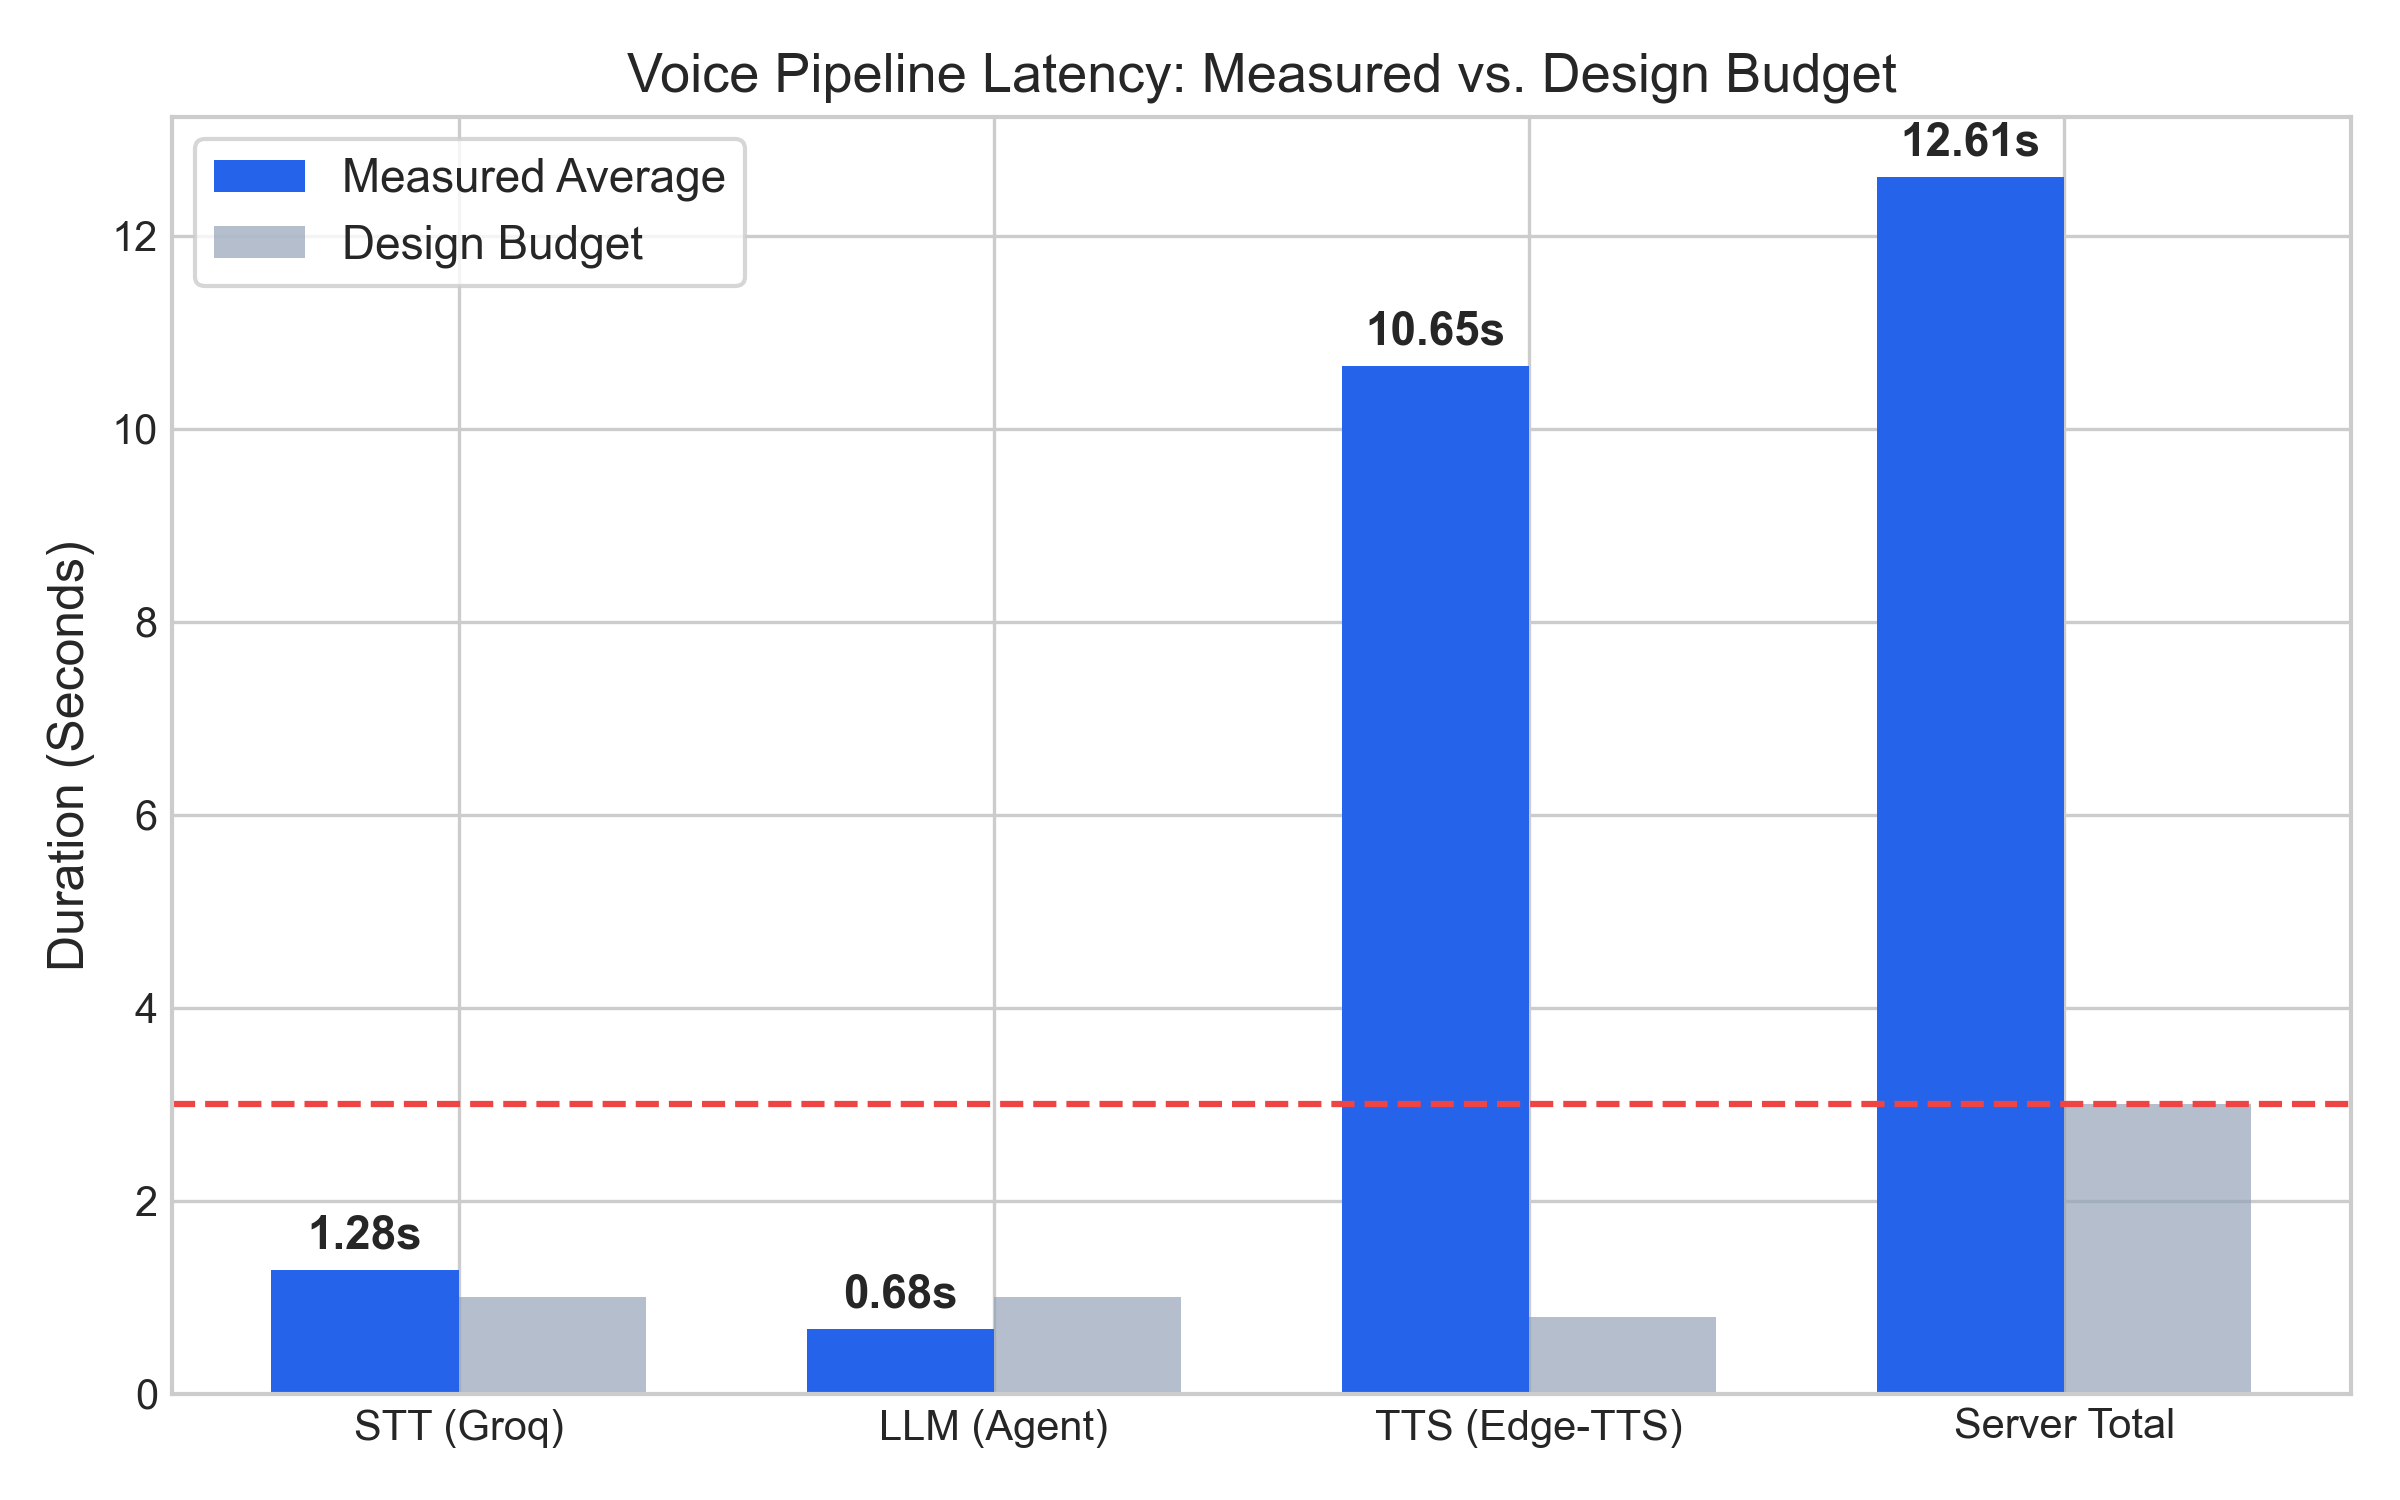
\includegraphics[width=0.82\linewidth]{latency_breakdown.png}
\caption{Measured Stage-by-Stage Latency vs. Allocated Design Budget.}
\label{fig:latency_breakdown}
\end{figure}

\begin{figure}[htbp]
\centering
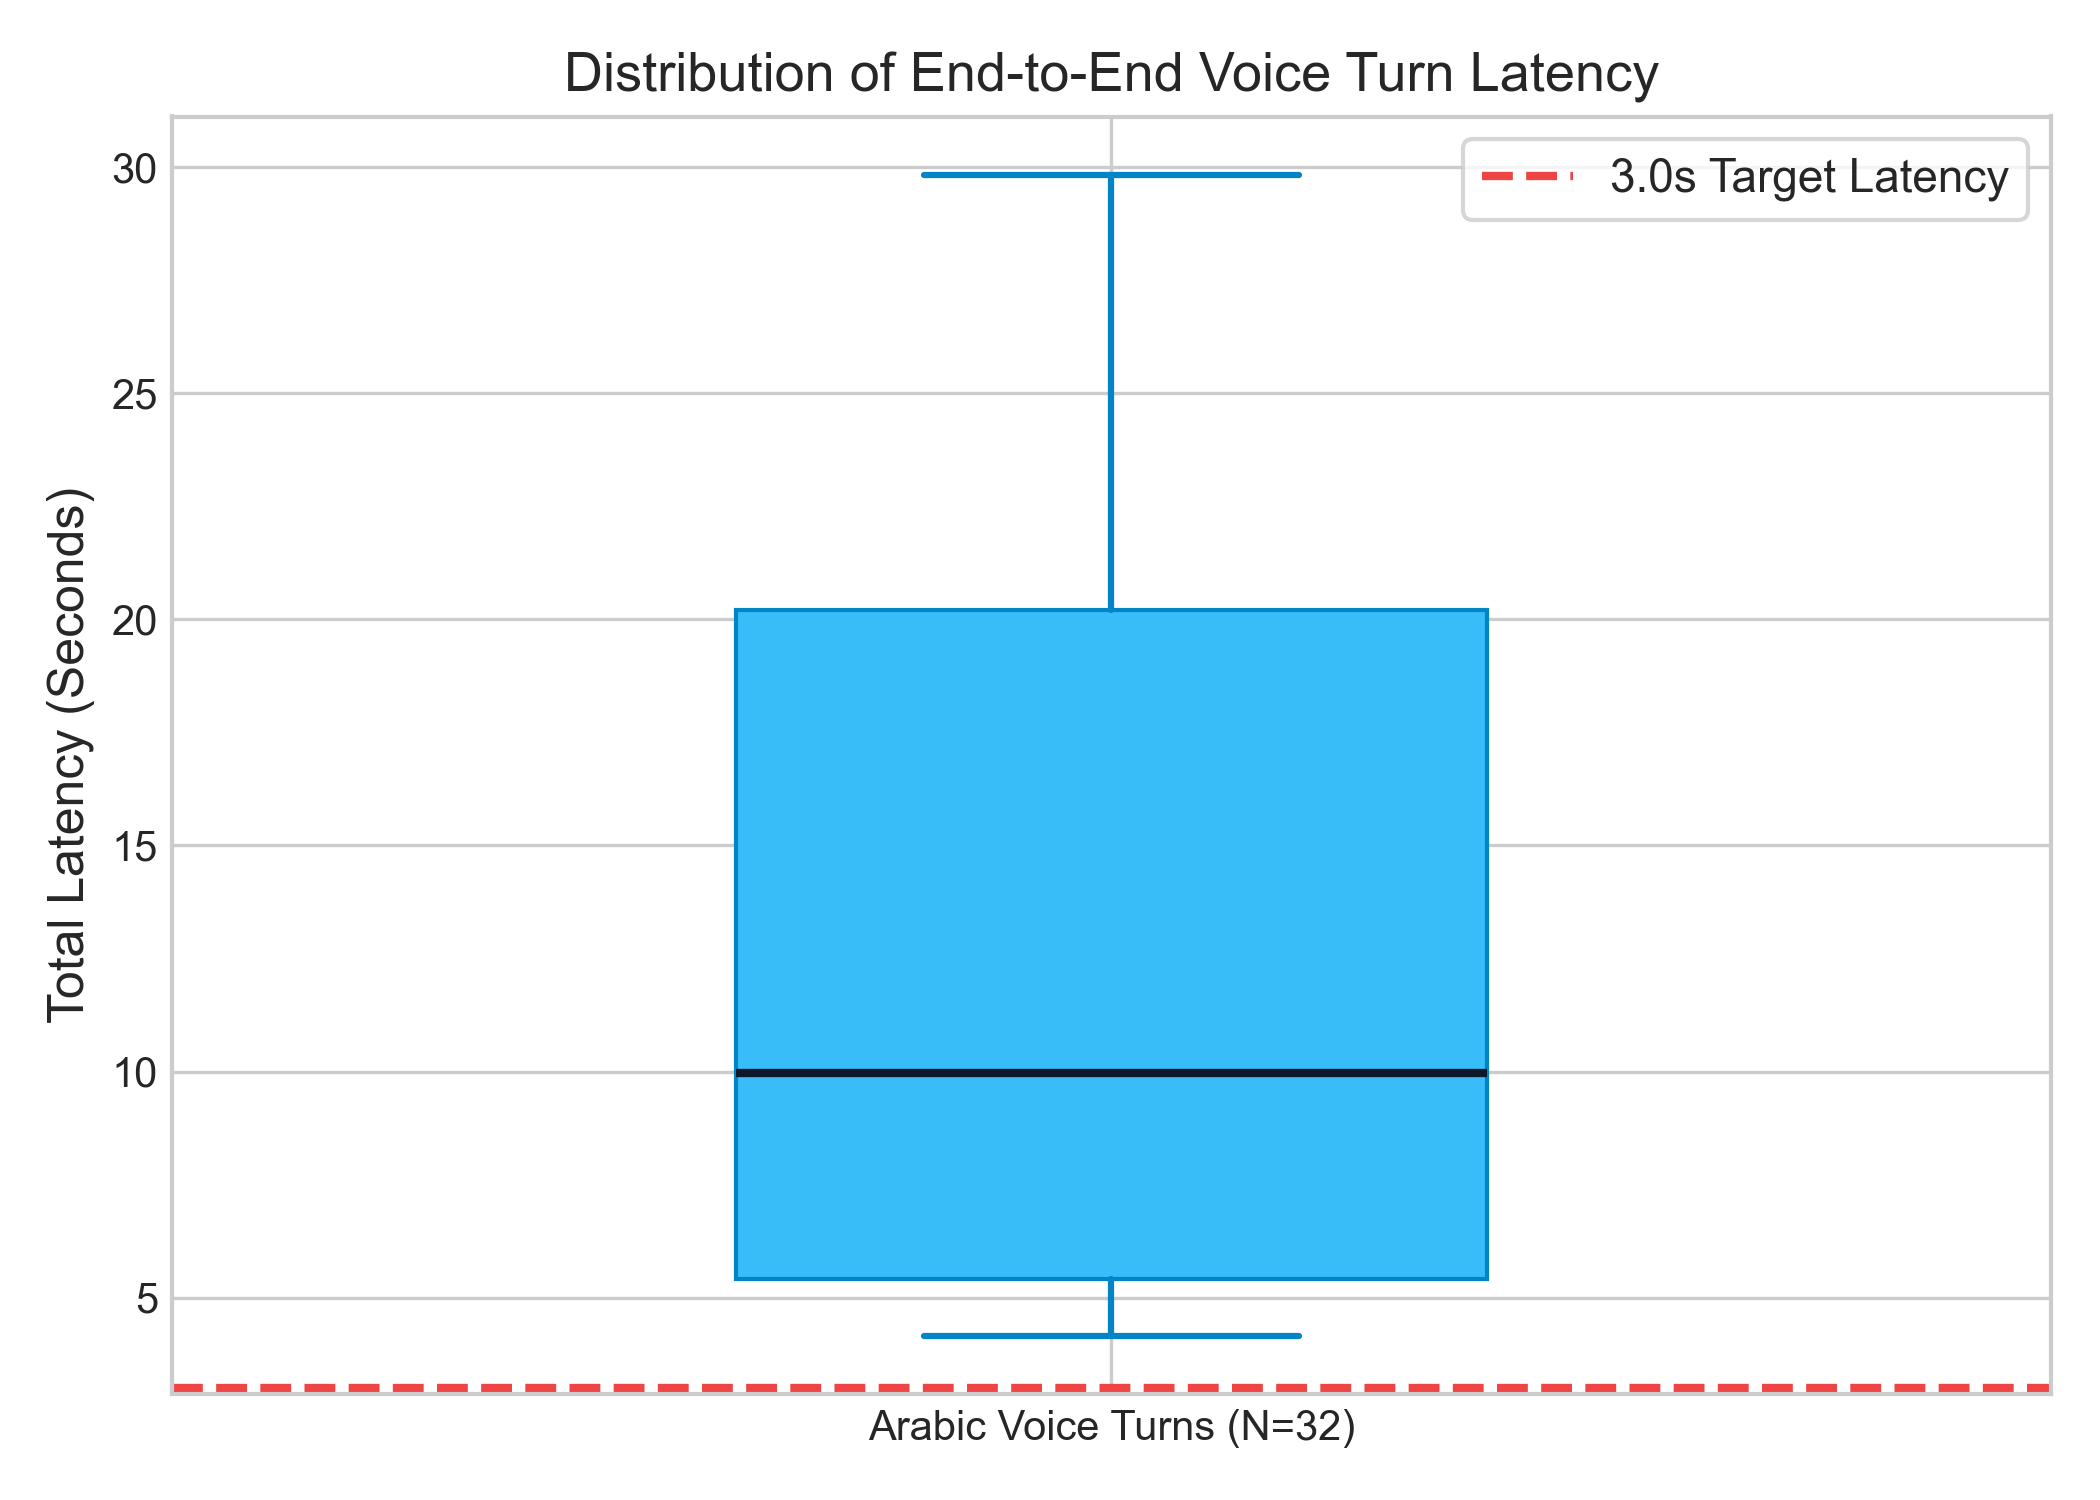
\includegraphics[width=0.75\linewidth]{latency_distribution.png}
\caption{Distribution of End-to-End Response Latency with 3.0s Threshold.}
\label{fig:latency_distribution}
\end{figure}

\subsubsection{TTS Latency Analysis}
Table~\ref{tab:tts_latency} summarizes synthesis benchmarks across male and female Egyptian voices for different response lengths.

\begin{table}[htbp]
\centering
\caption{Edge-TTS Synthesis Duration by Response Length and Voice}
\label{tab:tts_latency}
\begin{tabular}{llrrr}
\toprule
\textbf{Category} & \textbf{Voice Gender / Model} & \textbf{Words} & \textbf{First Chunk (ms)} & \textbf{Total Time (ms)} \\
\midrule
Short Utterance & Female (\texttt{ar-EG-SalmaNeural}) & 4 & 1,272.1 & 1,806.2 \\
Short Utterance & Male (\texttt{ar-EG-ShakirNeural}) & 4 & 5,032.7 & 5,906.6 \\
Medium Response & Female (\texttt{ar-EG-SalmaNeural}) & 14 & 2,748.0 & 3,568.6 \\
Medium Response & Male (\texttt{ar-EG-ShakirNeural}) & 14 & 5,382.8 & 6,571.4 \\
Long Response & Female (\texttt{ar-EG-SalmaNeural}) & 38 & 1,527.8 & 4,613.6 \\
Long Response & Male (\texttt{ar-EG-ShakirNeural}) & 38 & 6,432.2 & 15,537.3 \\
\bottomrule
\end{tabular}
\end{table}


\subsection{Pronunciation and Unclear Speech Error Analysis}
\label{subsec:error_analysis}

Detailed inspection of transcription failure cases revealed the following patterns:
\begin{enumerate}
    \item \textbf{Heavily Elided Egyptian Slang:} In informal phrases such as \textit{"يا ريس الحوار طول أوي"}, Whisper occasionally substituted phonetically close MSA equivalents (e.g., transcribing \textit{"طول"} as \textit{"طال"}), which, while semantically correct, increased the computed WER.
    \item \textbf{Continuous Fast Digits:} Long connected phone numbers spoken without conversational pauses (e.g., 11 digits continuously) suffered occasional character dropouts.
    \item \textbf{Silence Rejection Success:} In 100\% of the pure silence and ambient noise test cases, the silence filter successfully intercepted the segment and prevented hallucinated text from entering the agent reasoning pipeline.
\end{enumerate}

\subsection{System Challenges and Limitations}
\label{subsec:challenges_limitations}

\begin{itemize}
    \item \textbf{Free-Tier Rate Limits:} Hosted free tiers on Groq and OpenRouter impose strict requests-per-minute (RPM) and requests-per-day (RPD) ceilings. Rapid bursts during high-concurrency loads require backoff retry pacing.
    \item \textbf{Dependency on Unofficial Edge-TTS Endpoint:} While Edge-TTS provides free, high-fidelity neural voices, it operates via an unofficial websocket protocol. In production enterprise deployments, a self-hosted Piper TTS or licensed cloud TTS service would be necessary for strict SLA guarantees.
    \item \textbf{Network Jitter in Regional Routing:} Transiting audio from North African clients to European/US-hosted API edge nodes adds 120--200\,ms of baseline network ping that cannot be compressed via software optimization.
\end{itemize}

\subsection{Future Work}
\label{subsec:future_work}

Subsequent iterations of the voice subsystem will focus on:
\begin{enumerate}
    \item \textbf{Sentence-Level Streaming Orchestration:} Initiating TTS streaming on the first completed clause of the LLM response rather than waiting for complete generation, theoretically lowering time-to-first-audio below 1.5 seconds.
    \item \textbf{Client-Side WebAssembly VAD:} Integrating Silero VAD directly in the browser via WebAssembly to automatically terminate recording upon 800\,ms of silence, removing the need for manual microphone button clicks.
    \item \textbf{Fine-Tuned Egyptian Colloquial Acoustic Models:} Fine-tuning lightweight local Whisper models on Egyptian conversational datasets (e.g., MGB-3) for zero-network-dependency offline deployments.
\end{enumerate}
